\documentclass{standalone}
\usepackage{tikz}
\usetikzlibrary{arrows.meta, positioning, shapes.geometric, calc,patterns}

\begin{document}
	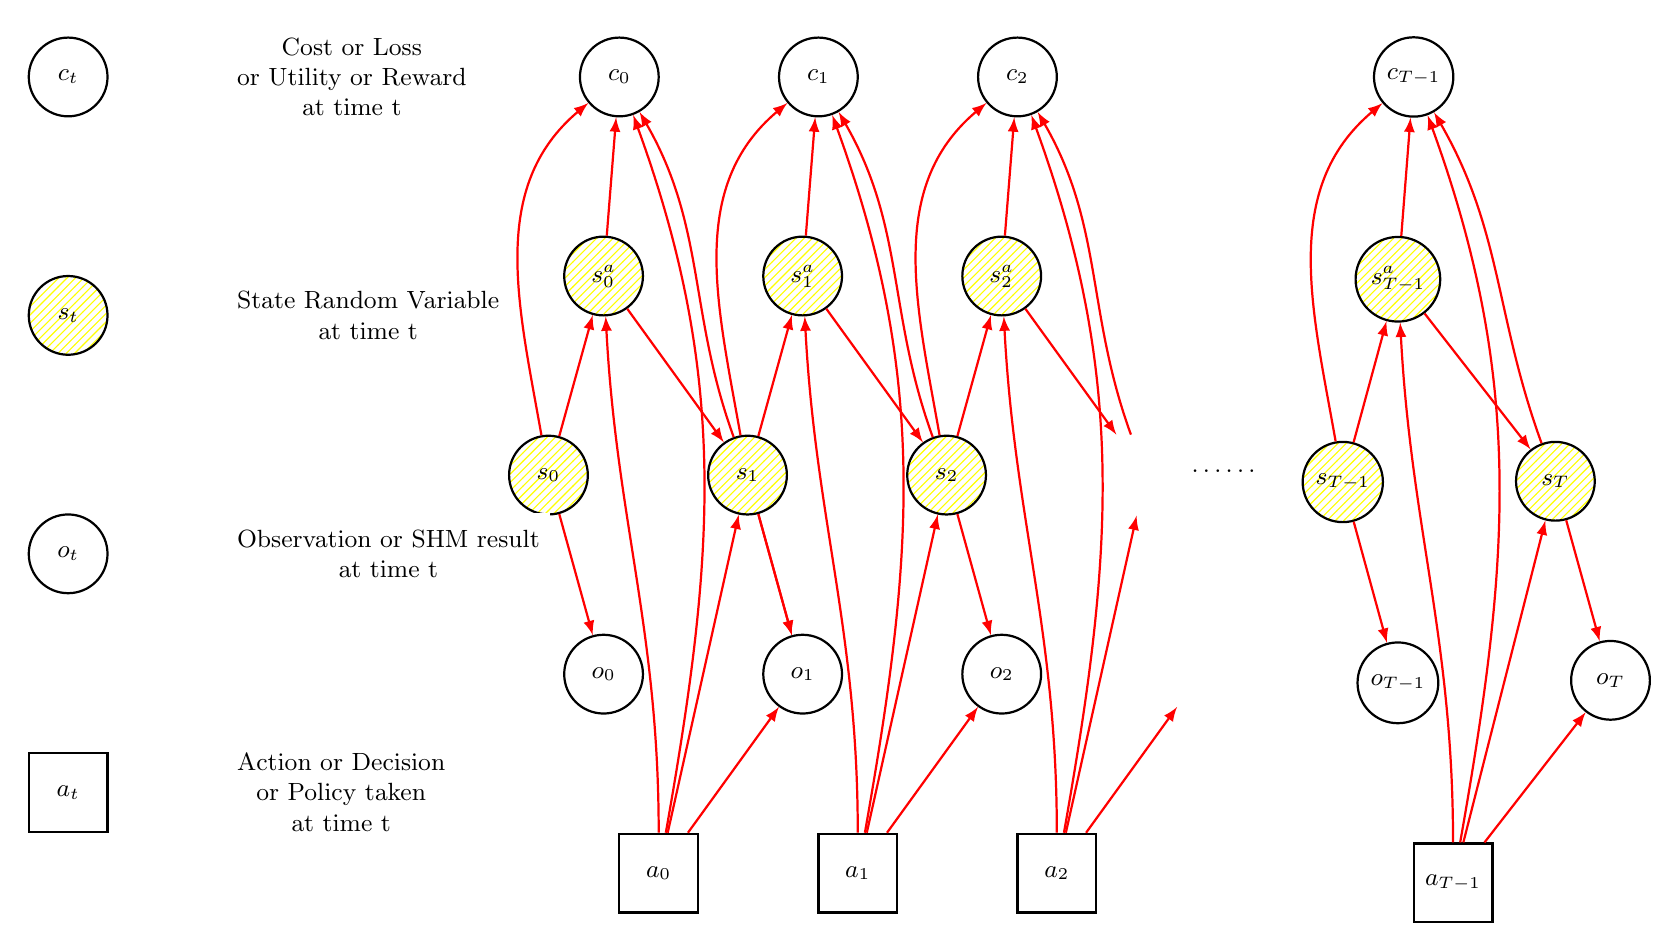
\begin{tikzpicture}[
		node distance=2cm and 1.5cm,
		every node/.style={draw, minimum size=10mm, font=\small},
		cost/.style={diamond, aspect=2, fill=white},
		cost/.style={circle, fill=white},
		shaded/.style={circle,pattern=north east lines, pattern color=yellow},
		obs/.style={circle, fill=white},
		action/.style={rectangle, fill=white},
		->, >=Stealth, thick, black
		]
		% Nodes for the first stage
		\node[cost] (c0) {$c_0$};
		\node[shaded, below=of c0, xshift=-2mm, yshift=+5mm] (s0a) {$s_0^{a}$};
		\node[shaded, below=of s0a, xshift=-7mm, yshift=+5mm] (s0) {$s_0$};
		\node[obs, below=of s0, xshift=7mm, yshift=+5mm] (o0) {$o_0$};
		\node[action, below=of o0, xshift=7mm, yshift=+5mm] (a0) {$a_0$};
		% Nodes for the second stage
		\node[cost, right=of c0] (c1) {$c_1$};
		\node[shaded, below=of c1, xshift=-2mm, yshift=+5mm] (s1a) {$s_1^{a}$};
		\node[shaded, below=of s1a, xshift=-7mm, yshift=+5mm] (s1) {$s_1$};
		\node[obs, below=of s1, xshift=7mm, yshift=+5mm] (o1) {$o_1$};
		\node[action, below=of o1, xshift=7mm, yshift=+5mm] (a1) {$a_1$};
		% Nodes for the third stage
		\node[cost, right=of c1] (c2) {$c_2$};
		\node[shaded, below=of c2, xshift=-2mm, yshift=+5mm] (s2a) {$s_2^{a}$};
		\node[shaded, below=of s2a, xshift=-7mm, yshift=+5mm] (s2) {$s_2$};
		\node[obs, below=of s2, xshift=7mm, yshift=+5mm] (o2) {$o_2$};
		\node[action, below=of o2, xshift=7mm, yshift=+5mm] (a2) {$a_2$};
		
		% Nodes for the third stage
		\node[draw = white, cost, right=of c2] (c3) {};
		\node[draw = white, fill = white, below=of c3, xshift=-2mm, yshift=+5mm] (s3a) {};
		\node[draw = white, fill = white, below=of s3a, xshift=-7mm, yshift=+5mm] (s3) {};
		\node[draw = white, obs, below=of s3, xshift=7mm, yshift=+5mm] (o3) {};
		\node[draw = white, action, below=of o3, xshift=7mm, yshift=+5mm] (a3) {};
		% Nodes for the final stage
		\node[cost, right=4cm of c2] (cT1) {$c_{T-1}$};
		\node[shaded, below=of cT1, xshift=-2mm, yshift=+5mm] (sT1a) {$s_{T-1}^{a}$};
		\node[shaded, below=of sT1a, xshift=-7mm, yshift=+5mm] (sT1) {$s_{T-1}$};
		\node[ obs, below=of sT1, xshift=+7mm, yshift=+5mm] (oT1) {$o_{T-1}$};
		\node[shaded, below=of sT1a, xshift=+20mm, yshift=+5mm] (sT) {$s_T$};
		\node[obs, below=of sT, xshift=+7mm, yshift=+5mm] (oT) {$o_T$};
		\node[action, below=of oT1, xshift=7mm, yshift=+5mm] (aT1) {$a_{T-1}$};
		
		\node[draw = white] at (7.7,-5) {\dots \dots};
		
		% Arrows for first stage
		\draw[-latex,thick,red] (s0) -- (s0a);
		\draw[-latex,thick,red] (s0) to[out=100,in=220] (c0);
		\draw[-latex,thick,red] (s0) -- (o0);
		\draw[-latex,thick,red] (s0a) -- (c0);
		\draw[-latex,thick,red] (a0) to[out=90,in=-87] (s0a);
		\draw[-latex,thick,red] (a0) to[out=80,in=-70] (c0);
		\draw[-latex,thick,red] (a0) -- (s1);
		\draw[-latex,thick,red] (a0) -- (o1);
		\draw[-latex,thick,red] (s1) to[out=110,in=-60] (c0);
		\draw[-latex,thick,red] (s0a) -- (s1);
		\draw[-latex,thick,red] (s1) -- (o1);
		
		\draw[-latex,thick,red] (s1) to[out=100,in=220] (c1);
		\draw[-latex,thick,red] (s1) -- (s1a);
		\draw[-latex,thick,red] (s1a) -- (c1);
		\draw[-latex,thick,red] (s1) -- (o1);
		\draw[-latex,thick,red] (s1a) -- (s2);
		\draw[-latex,thick,red] (a1) to[out=90,in=-87] (s1a);
		\draw[-latex,thick,red] (a1) to[out=80,in=-70] (c1);
		\draw[-latex,thick,red] (a1) -- (s2);
		\draw[-latex,thick,red] (a1) -- (o2);
		\draw[-latex,thick,red] (s2) to[out=110,in=-60] (c1);
		
		
		
		
		
		\draw[-latex,thick,red] (s2) to[out=100,in=220] (c2);
		\draw[-latex,thick,red] (s2) -- (s2a);
		\draw[-latex,thick,red] (s2a) -- (c2);
		\draw[-latex,thick,red] (s2) -- (o2);
		\draw[-latex,thick,red] (s2a) -- (s3);
		\draw[-latex,thick,red] (aT1) to[out=90,in=-87] (sT1a);
		\draw[-latex,thick,red] (aT1) to[out=80,in=-70] (cT1);
		\draw[-latex,thick,red] (aT1) -- (sT);
		\draw[-latex,thick,red] (aT1) -- (oT);
		\draw[-latex,thick,red] (s3) to[out=110,in=-60] (c2);
		
		\draw[-latex,thick,red] (a2) to[out=90,in=-87] (s2a);
		\draw[-latex,thick,red] (a2) to[out=80,in=-70] (c2);
		\draw[-latex,thick,red] (a2) -- (s3);
		\draw[-latex,thick,red] (a2) -- (o3);
		
		\draw[-latex,thick,red] (sT1) -- (sT1a);
        \draw[-latex,thick,red] (sT1a) -- (sT);	
		\draw[-latex,thick,red] (sT1a) -- (cT1);
		\draw[-latex,thick,red] (sT) -- (oT);
		\draw[-latex,thick,red] (sT1) -- (oT1);
		\draw[-latex,thick,red] (sT) to[out=110,in=-60] (cT1);
		\draw[-latex,thick,red] (sT1) to[out=100,in=220] (cT1);
		
		% Denote 
		\node[cost] at (-7,0) (costnode) {$c_t$};
		\node[draw = white,right= of costnode,align=center]  {Cost or Loss \\ or Utility or Reward \\at time t};
		\node[shaded, below = of costnode] (statenode) {$s_t$};
		\node[draw = white, right = of statenode,align = center] {State Random Variable \\ at time t};
		\node[obs, below= of statenode]  (obsnode) {$o_t$};
		\node[draw = white, right = of obsnode,align = center]  {Observation or SHM result \\ at time t};
		\node[action,below = of obsnode]  (actionnode) {$a_t$};
		\node[draw = white, right = of actionnode, align=center] {Action or Decision \\or Policy taken \\ at time t};
%		\draw (s0_a) -- (s0);
%		\draw (s0) -- (O0);
%		\draw (s0_a) -- (O0);
%		\draw (s0) -- (A0);
%		\draw (O0) -- (A0);
%		
%		% Arrows for second stage
%		\draw (C1) -- (s1_a);
%		\draw (C1) -- (s1);
%		\draw (s1_a) -- (s1);
%		\draw (s1) -- (O1);
%		\draw (s1_a) -- (O1);
%		\draw (s1) -- (A1);
%		\draw (O1) -- (A1);
%		
%		% Arrows for third stage
%		\draw (C2) -- (s2_a);
%		\draw (C2) -- (s2);
%		\draw (s2_a) -- (s2);
%		\draw (s2) -- (O2);
%		\draw (s2_a) -- (O2);
%		\draw (s2) -- (A2);
%		\draw (O2) -- (A2);
%		
%		% Arrows for final stage
%		\draw (CT) -- (ST1_a);
%		\draw (CT) -- (ST);
%		\draw (ST1_a) -- (ST);
%		\draw (ST) -- (OT);
%		\draw (ST1_a) -- (OT);
%		\draw (ST) -- (AT1);
%		\draw (OT) -- (AT1);
%		
%		% Inter-stage arrows
%		\draw (s0) to[out=10,in=170] (C1);
%		\draw (A0) to[out=10,in=170] (C1);
%		\draw (O0) to[out=10,in=170] (C1);
%		
%		\draw (s1) to[out=10,in=170] (C2);
%		\draw (A1) to[out=10,in=170] (C2);
%		\draw (O1) to[out=10,in=170] (C2);
%		
%		\draw (s2) to[out=10,in=170] (CT);
%		\draw (A2) to[out=10,in=170] (CT);
%		\draw (O2) to[out=10,in=170] (CT);
%		
%		% Dotted line separation
%		\draw[dashed] ($(C2.east)+(1.2,1.5)$) -- ($(AT1.south)+(1.2,-0.5)$);
		
	\end{tikzpicture}
\end{document}
